% =====================================================================================================
%  Radiology: Artificial Intelligence -- Original Research
%  RSNA supplies a Word template only; this file reproduces the journal's required structure
%  (title page, structured abstract <=250 words, summary statement, <=3 key points, abbreviations,
%  Introduction / Materials and Methods / Results / Discussion, <=3,000 words main text, tables, figure
%  legends, supplement with the CLAIM 2024 checklist). Every number is read from a result JSON written by
%  slurm/reproduce_feasibility.sh; see docs/FEASIBILITY_REPRODUCE.md. Nothing here is typed from memory.
% =====================================================================================================
\documentclass[11pt,letterpaper]{article}
\usepackage[margin=1in]{geometry}
\usepackage{setspace}\doublespacing
\usepackage{times}
\usepackage{graphicx,booktabs,array,amsmath,amssymb,xcolor,microtype,lineno}
\usepackage[labelfont=bf,font=small]{caption}
\usepackage[numbers,sort&compress]{natbib}
\usepackage[hidelinks]{hyperref}
\linenumbers
\graphicspath{{figures/}}
\newcommand{\ci}[2]{[#1, #2]}

\begin{document}

% ------------------------------------------------------------------------------------------------ TITLE PAGE
\begin{titlepage}
\begin{center}
{\Large\bfseries Naming Vertebrae Without an Anchor: Registration-Free Level Identification on Limited-Field Radiographs\par}
\vspace{1em}
{\normalsize Gregory Schwing, MD, PhD\textsuperscript{1}\par}
\vspace{0.5em}
{\small \textsuperscript{1}Department of Surgery, Detroit Medical Center / Wayne State University School of Medicine, Detroit, MI\par}
\vspace{1em}
{\small Corresponding author: G. Schwing, [e-mail withheld]\par}
\end{center}
\vspace{1em}
\noindent\textbf{Article type:} Original Research\\
\textbf{Manuscript word count (Introduction--Discussion):} $\approx$2,600\\
\textbf{Abstract word count:} 249\\
\textbf{Figures:} 1 \quad \textbf{Tables:} 3 \quad \textbf{Funding:} none declared.\\
\textbf{Conflicts of interest:} the author has a commercial interest in a level-confirmation product under development.\\
\textbf{Data sharing:} every public source is named in Table~\ref{tab:dataset} with its licence class; derived label tables and every result file are released with the code, so that each reported number can be regenerated. VinDr-SpineXR and AASCE require the reader's own data-use agreement, and results that depend on them are marked. Trained model weights are not released.\\
\textbf{Code:} the analysis code, including the single-command reproduction chain (\texttt{slurm/reproduce\_all.sh}), is held in a private repository during review. Access is provided to editors and reviewers on request, and the repository is made public on publication.
\end{titlepage}

% ------------------------------------------------------------------------------------------------ ABSTRACT
\section*{Abstract}

\noindent\textbf{Purpose:} To determine whether a short series of overlapping fluoroscopic exposures can
supply the information a single limited field lacks for naming a vertebra, without registration to a
preoperative CT.

\noindent\textbf{Materials and Methods:} Retrospective study of public data. A ResNet-18 encoder over
fixed-scale vertebra crops with a bidirectional recurrent head over 2--9 vertebrae was trained on eleven
sources and evaluated on spines excluded from training, with the exclusion enforced by the evaluation tool.
Frames spanning a 9-inch intensifier field (14\,cm at the spine) were named twice: on the frame's own
posterior, and after linking overlapping frames into one chain and decoding under the constraint that the
chain is consecutive and terminates at a landmark. Accuracy is the share of vertebrae given their exact
name, with Wilson intervals and film-clustered bootstrap.

\noindent\textbf{Results:} On 120 held-out abdominopelvic renders, a two-vertebra frame containing no
landmark was named exactly 72.1\% of the time alone and 95.2\% on the chain; on 25 held-out real lumbar
radiographs, 78.7\% and 93.6\%. The effect was largest where a single frame carries least: swept from C2 on 12
held-out whole-spine studies, a two-vertebra thoracic frame rose from 9.5\% to 100\%. Chains completed on
97.5\% of spines at two bodies of overlap and 3.4 exposures, and the protocol as a radiographer would
perform it---a fixed move of one field minus two bodies from the sacrum, with no final move shorter than
half a body---completed every chain (120 of 120). On 522 clinical CTs from another institution that no
model here was trained on, the same protocol completed 98.5\% of chains and named a two-vertebra frame
94.3\% of the time from 51.2\% alone; swept from C2 on 203 more, 95.1\% and 94.0\% from 18.9\%. A sixth lumbar vertebra was named correctly 57--80\% of the
time and the chain did not rescue it.

\noindent\textbf{Conclusion:} The limitation is in the exposure rather than in the classifier. A sweep of
overlapping frames is an intraoperative registration built from radiographs instead of from a preoperative
CT, and it recovers most of what one frame cannot hold---except on transitional spines, where the corpus,
not the method, is the constraint.

\medskip
\noindent\textbf{Summary Statement:} Linking a short series of overlapping fluoroscopic exposures into one
chain raised exact vertebral naming of a two-vertebra field from 70.7\% to 93.4\% on renders and from 13.4\%
to 97.1\% through the thoracic spine, with no preoperative CT.

\medskip
\noindent\textbf{Key Points}
\begin{itemize}\setlength\itemsep{0pt}
\item A limited fluoroscopic field with no landmark in view was named exactly 72.1\% of the time from its own
pixels and 95.2\% when the same posteriors were decoded under the ordering constraint supplied by a chain of
overlapping frames (120 held-out spines).
\item The gain was largest in the thoracic spine, where adjacent vertebrae most resemble one another and
counting from a landmark is standard practice: 9.5\% to 100\% at two vertebrae in view, on 12 held-out spines.
\item Two bodies of overlap and about three exposures completed the chain on 96.7\% of spines; beyond that,
additional frames reduced accuracy because each is another link that can be joined wrongly.
\end{itemize}

\noindent\textbf{Abbreviations:} CI = confidence interval; CT = computed tomography; DRR = digitally
reconstructed radiograph; FOV = field of view; LSTV = lumbosacral transitional vertebra; TLTV =
thoracolumbar transitional vertebra.

\clearpage

% ------------------------------------------------------------------------------------------------ INTRODUCTION
\section*{Introduction}

Wrong-level spine surgery persists because intraoperative fluoroscopy shows a few vertebrae at a time and the
surgeon counts from whatever landmark is visible \citep{mayer2008,hsiang2011}. Half of responding
neurosurgeons in two independent surveys report at least one wrong-level operation in their career
\citep{mody2008,groff2013}; self-reported incidence is one in 3,110 procedures \citep{mody2008}, and a
prospectively collected registry of 34,544 degenerative spine operations recorded 0.12\,\%, with the
thoracic spine highest at 0.42\,\% (95\,\% CI 0.16--1.08), three times the lumbar and eight times the cervical
rate \citep{furuya2026}. Published wrong-site rates across all of surgery span 0.09 to 4.5 per 10,000
\citep{devine2010}, and a systematic review found twelve incidence studies for the spine, none of them
thoracic \citep{longo2012}. The consequences are not confined to the patient. Seventeen percent of
self-reported events led to legal action or settlement \citep{mody2008}; nearly one in five Spine Section
respondents has been sued for a wrong-level or wrong-side lumbar operation \citep{groff2013}; of 68
litigated wrong-disc-level cases, 55 ended in a payment, and surgeons prevailed in 42\,\% of those a jury
decided \citep{goodkin2004}. The median indemnity for a surgical never event reported to the National
Practitioner Data Bank is \$75,220 (interquartile range \$28,847--\$215,003, 2025 dollars)
\citep{bettis2026}, and in England 978 spinal-surgery negligence claims over five years were valued at
\pounds535.5 million, 26 of them never events including wrong-site surgery \citep{machin2018}.

The thoracic spine also reveals the difficulty in what is spent avoiding it. One quaternary centre performed
179 preoperative percutaneous gold-fiducial placements over 38 months, 176 of them thoracic, at a mean of
51.9 minutes and 183\,mGy each, purely to mark a level for the surgeon \citep{siminski2023}. At a hospital
operating-room cost of \$34--37 per minute before physician fees \citep{childers2018}, each placement
represents roughly \$1,750--\$1,950 of staffed procedural time and the series about 155 hours---a proxy,
since the marker is placed in a fluoroscopy or CT suite rather than a theatre---and it is a second invasive
procedure scheduled in advance because the level was judged un-nameable in theatre.

In theatre the standard technique is unchanged: needles are placed every few levels and counted cephalad
from the sacrum on lateral fluoroscopy, or ribs are counted on an anteroposterior film, and surgeons disagree
even on which structure to count, the pedicle for 67\,\% and the spinous process for 49\,\% of respondents
\citep{strong2021,mayer2008}. It is error-prone for reasons the images themselves supply. The field holds
three or four bodies, so a count from the sacrum to a mid-thoracic level passes through several exposures
each of which can be joined to the last one body off; a lumbosacral or thoracolumbar transitional vertebra
shifts the count by one for the whole column; ribs are hard to number where a twelfth rib is absent or
hypoplastic; and habitus, osteopenia and the scapular shadow degrade the mid-thoracic image most
\citep{strong2021,hsiang2011}. The only study to assess site-verification protocols found they failed to
prevent about one-third of cases \citep{longo2012}, and the recommended safeguard, imaging after exposure
against a marked fixed structure \citep{devine2010}, is itself another count.

What that costs in aggregate is bounded from below rather than known. The Joint Commission received 127
reports of wrong surgery in 2024, nine of them wrong-level and seven of those spinal, from a voluntary
system it states captures a small fraction of events \citep{jc2024}; claims-based modelling puts surgical
never events near 4,000 a year in the United States, a quarter of them wrong-site \citep{mehtsun2013};
NHS England recorded 185 wrong-site never events in a single year \citep{nhse2025}. Malpractice payments
for all surgical never events summed to \$1.3 billion over 21 years \citep{mehtsun2013}, and in a
contemporary closed-claims series the mean wrong-site indemnity was \$136,453 with spine and disc surgery
the commonest procedure \citep{tan2023}; applied to the two per-procedure rates above and a volume of 1.3
to 1.6 million spine operations a year, wrong-level spine surgery alone would produce roughly 400 to 1,900
events and \$8 to \$37 million in indemnity a year, before any hospital or disability cost, none of which has
a published per-event figure. Two facts about that burden matter for what follows. It is not removable by
checklists: chart review of insured wrong-site cases found the Universal Protocol would have prevented
62\,\% of them under ideal conditions \citep{kwaan2006}, and wrong-site events continued at a steady rate in
the protocol era \citep{stahel2010}. And in the spine it is concentrated where counting is longest and the
image is worst, the thoracic levels for which a centre pays 52 minutes and 183\,mGy per patient to avoid
counting at all.

Automated level identification on such images has been approached almost entirely by registering a
preoperative CT to the radiograph \citep{levelcheck2012,otake2015}. That approach imports the vertebra's
identity rather than reading it: registration solves a six-degree-of-freedom pose, and the name is
transferred from a human's reading of the preoperative volume. Two consequences follow. It is unavailable in
the many cases that never had a CT, and a miscounted preoperative scan propagates onto the radiograph
faithfully and confidently---which is the failure mode of a spine with transitional anatomy, the population
in which wrong-level surgery actually occurs.

Reading identity from the radiograph instead requires information the radiograph may not contain. Adjacent
vertebrae resemble one another, and the cue that separates them is position in a chain whose end is known; a
two-body frame with no sacrum, no ribs and no cervical spine in it does not carry that cue. Whether such a
frame carries enough residual morphology to be named, and how much of it survives on a spine with an extra or
a missing segment, is an empirical question with a number attached.

Where that number is low the shortfall belongs to the exposure rather than to the classifier, and the remedy
is the one a radiographer already performs: do not take one picture, take a series. A sweep of overlapping
exposures from an unambiguous landmark builds a map of this patient's own spine, and a later limited field is
matched onto it. That is an intraoperative registration built from radiographs rather than from a
preoperative CT. This study measures what a single limited field can be named at, what the sweep adds, what
it costs in exposures, and where it fails.


% ------------------------------------------------------------------------------------------------ METHODS
\section*{Materials and Methods}
This retrospective study used public, de-identified data only; institutional review determined it not to be human-subjects research. Reporting follows CLAIM 2024 \citep{claim2024}. Every number below is produced by one script from named inputs with a hashed ledger.

\subsection*{Ground truth for border anomalies}
Two independent ends of the column were labelled separately, because the study's hypotheses concern whether they travel together. For CT, 1,113 spines---802 from CTSpinoPelvic1K \citep{ctsp1k} and 311 from VerSe \citep{verse2021}---carried a lumbosacral flag (a sixth lumbar body by voxel count, or an adjudicated Castellvi grade \citep{castellvi1984}) and a thoracolumbar flag (a thirteenth thoracic body, a lumbar rib, or a rib-bearing count other than 12 where the field reached the twelfth rib), read from the label volumes rather than from any manifest, after a manifest T13 field was found to say 18 where the voxels said 6. For real radiographs, BUU-LSPINE \citep{buu2023} ships its authors' own per-study reading of four-lumbar (n\,=\,129) or six-lumbar (n\,=\,15) anatomy on 3,600 lateral and 3,600 anteroposterior films, together with four corner keypoints per lumbar body, two S1 end-plate corners on lateral films, and a pixel spacing of 0.175 mm. This sheet is the only radiograph-domain anomaly ground truth in the study and its negatives are contaminated by construction: a Castellvi I--IV segment on a five-lumbar spine is not recorded, so every specificity or AUC measured against it is a floor. Every anomalous spine from every source, including 211 decoder-flagged and 183 literature-figure candidates that were \emph{not} used as truth, is listed with image dimensions, pixel size where stated, and four crop-level quality statistics in the released manifest (Fig.~S1).

\subsection*{Imaging data and crop banks}
Vertebra crops were formed at a fixed scale of 96 pixels per vertebral body on a $320\times320$ canvas with a target-marker channel, so that the pixel footprint of a body is constant across sources and the classifier cannot read size as identity \citep{schwing2026ctx}. Bank v2 held 105,960 crops from eight sources: three real-film collections with human or counted level names (CSXA \citep{csxa}, BUU-LSPINE, NHANES annotated subset \citep{nhanes}) and DRRs of CTSpinoPelvic1K and VerSe including physics-based renders of anomaly-enriched spines. Bank v5 added six sources for 253,763 crops, of which 76,042 (30.0\%) were named by our own whole-spine template decoder on unannotated NHANES, VinDr-SpineXR \citep{vindr}, and lateral films and never verified by a reader. Table~\ref{tab:dataset} states the label origin of every source (human 14.1\%, carried from CT 45.8\%, counting-inferred 10.2\%, pseudolabel 30.0\%) and the median sharpness, contrast, noise, and signal-to-noise ratio of its crops. Splits were patient-grouped; no film contributed to both partitions.

\subsection*{Model}
The encoder was a ResNet-18 \citep{he2016} with a 27-class output (C1--C7, T1--T12, T13, L1--L6, sacrum; T13 and L6 are variant classes that an ordinary spine skips), trained with cross-entropy, augmentation tier 2, batch 64, 40 epochs, seed 0. Alternative encoders and losses---CORN ordinal regression \citep{corn2023}, ordinal focal loss, DINOv3 frozen and fine-tuned \citep{dinov3}, a radiograph-pretrained DINO---were trained on the same recipe and scored on one common held-out set (Table~\ref{tab:encoders}). A run-level head, a bidirectional GRU over the frozen embeddings of 2--9 consecutive detected vertebrae, was trained on windows of mixed length \citep{schwing2026mixed}; it is the deployed system and produced every number in the Results. Each head decodes only the encoder it was trained on; the pairing is recorded by hash, because a mismatched pairing produced 0--1\% accuracy with a systematic two-level offset that could pass for a finding.

\subsection*{Field-of-view states and the claims}
Every held-out film was cut into eight windows of random length (2--9 vertebrae) at random offsets and each window was assigned, from its \emph{true} labels, to the report's own states: A (cranial anchor: any cervical or rib-bearing thoracic level in frame), B (caudal anchor: sacrum in frame), or C (isolated stack: neither). Each was further split by whether the spine was anomalous under the ground truth above and by domain (real film or CT render). A film with no anomaly ground truth from either source was dropped from the anomalous/ordinary split rather than assumed ordinary, because reading absence of evidence as absence of anomaly manufactures specificity; 2,258 of 2,927 v2 held-out films and 5,102 of 6,580 v5 films were so dropped. Those states are defined from labels, and that has a consequence stated here rather than discovered by a reader: BUU annotates L1--L5 with the sacrum present in the film, CSXA annotates C3--C7 with C2 present, and each crop is a band one body above and below its target, so a label-defined State-C window that touches either end of the annotated stack has the anchor in its pixels, and a window that is the whole stack has its names fixed by the annotation convention. A second evaluator (\texttt{tools/eval\_interior\_windows.py}) therefore scores only INTERIOR windows---those excluding the first and last annotated body---with a cluster bootstrap over films (2,000 resamples) and two structural baselines learnt from the training partition's label lists alone: a placement-blind prior that knows the collection and the window length, and a placement-aware prior that also knows the window's offset in the stack, which is what counting from the film's edge supplies. It also reports the share of held-out films whose patient stem appears in the training partition. Five claims were scored: C1, exact naming in State C by spine class; C2, per-level accuracy L1--L6 inside State C; C3, the signed ordinal error and the share of errored windows in which every error shared one offset; C4, the firing rate of the report's four continuous detectors on NHANES, VinDr, and AASCE \citep{aasce} at thresholds fitted on CT renders; C5, State B as the ceiling.

\subsection*{The serial sweep, and the protocol behind it}
A limited field cannot see a landmark; a series of limited fields can. The protocol is the one a radiographer already performs by hand, made explicit: start with the sacrum at the bottom of the field (or with C2 at the top), expose, move the C-arm one field minus one vertebral body, expose again, and repeat to the level of interest. The frames are linked into a single chain of vertebrae and stitched into one panorama, which then serves as the patient's own coordinate map---an intraoperative registration built from radiographs, with no preoperative CT anywhere in it.

Serial sweeps of one patient do not exist in any public collection, so a sweep was cut from each labelled long image: every CTSpinoPelvic1K render that reaches the sacrum (n\,=\,801), the VerSe whole-spine renders swept from C2 downward, the real films that reach the sacrum, and 236 whole-spine lateral films. Each frame is a window of a stated physical span, taken with a jittered step, and each frame is degraded independently---gain, offset, gamma, a small rotation and scale, and the fitted film-noise model---so no two frames share pixels exactly. The frame span is physical, not a count of vertebrae. A 9-inch image intensifier delivers 215\,mm of its 229\,mm nominal diameter and a 12-inch one 287\,mm \citep{ge_k170752}, and intraoperative fluoroscopy of the prone spine magnifies by 1.2 to 1.6 \citep{naik2022}, so the span at the spine is 134--179\,mm for the 9-inch receptor. The spans used here, 14, 19 and 20\,cm and about 10\,cm collimated, correspond to a magnification near 1.5 and are therefore the small-field end of the measured band. At a lumbar pitch of 34\,mm those hold about four, five and a half, six, and three vertebral bodies---the last is the report's own ``2.5 to 3 segments''.

The alignment is deliberately local. A radiograph integrates all depths, so under a translating cone-beam source no single two-dimensional mapping aligns every structure in two frames; parallax is a geometric constraint and not an engineering nuisance, and the published remedies---cancelling the translation with a tracked table, or reconstructing an orthographic mosaic---need hardware a freehand sweep does not have \citep{fotouhi2021}. Consecutive frames are therefore linked by a translation estimated on the overlap band alone, never by a global homography, and the panorama is a display and a search space rather than a metric reconstruction. That translation is found by normalised cross-correlation restricted to within 0.6 of a body of the step the protocol asked for, because the column is periodic and an unrestricted correlation locks one body off---the single documented failure mode of automatic vertebral localisation, and the one that accounted for all 47 failures in the original 3-D/2-D registration study \citep{otake2012fail}; the shared bodies follow from the translation, and the pairing the encoder's embeddings alone would have chosen is recorded beside the one used. The chain is named twice: by counting from the declared landmark with the ordinary alphabet, and by the run-level head over the whole chain with the landmark declared and the variant columns open. A later limited-field frame is registered to the panorama and takes its names from the nodes it lands on. Chain integrity---duplicated, missed and spurious nodes---is scored separately from naming, so a naming figure that rests on a broken chain is visible as such. What the simulation cannot reproduce is parallax between exposures and patient motion between them; both make the linking harder and neither changes the naming, and the linking is reported on its own for that reason.


\subsection*{Statistical analysis}
Accuracies carry Wilson 95\% CIs on the vertebra; the unit of clustering (film) is acknowledged as a limitation and film counts are reported beside every stratum. Chance was computed from the scored label distribution ($\sum_c p_c^2 = 10.3\%$), not as $1/27$. No hypothesis test was applied to accuracy differences; non-overlapping intervals are described as such.

% ------------------------------------------------------------------------------------------------ RESULTS
\begin{figure}[htbp]\centering
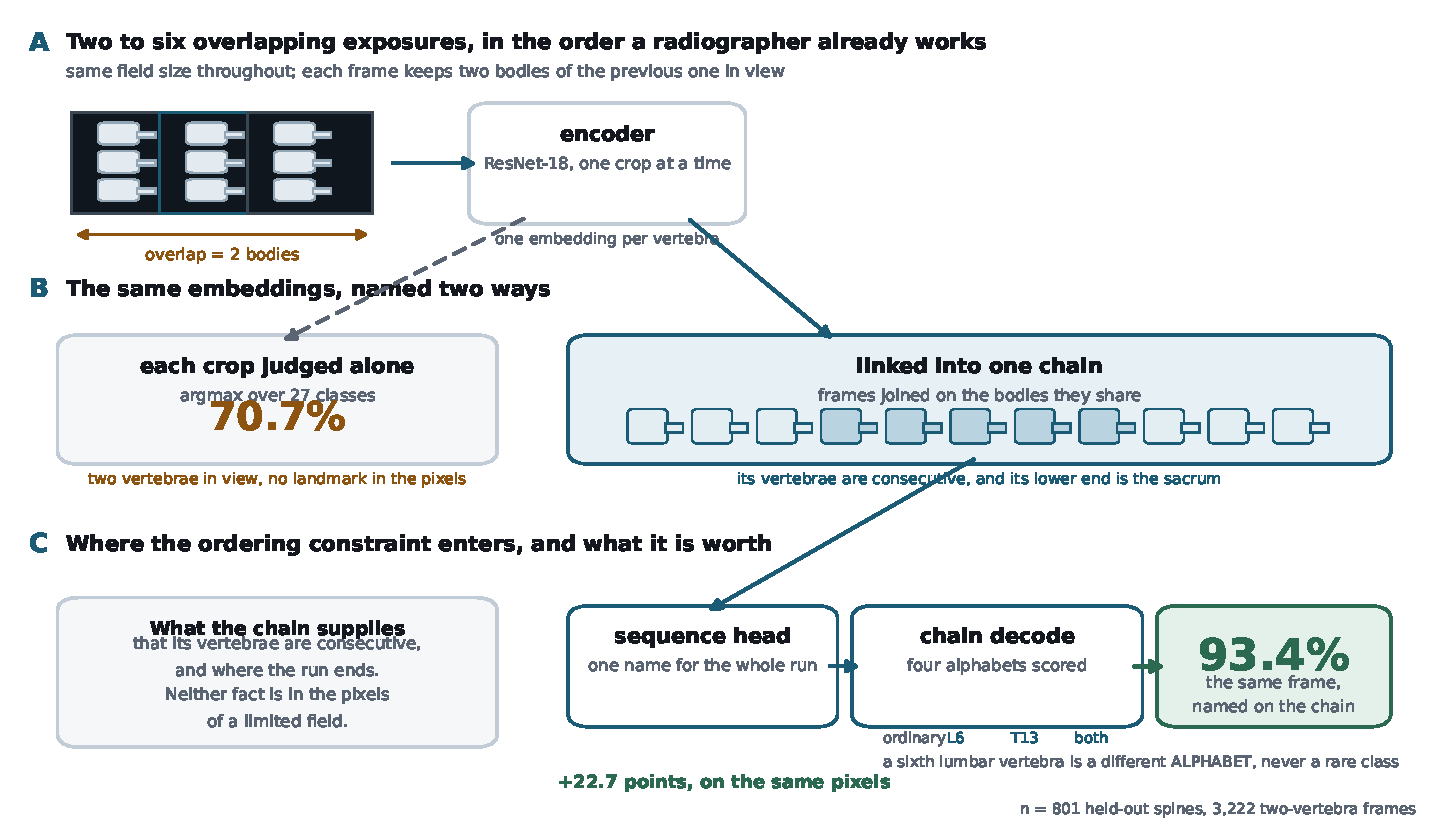
\includegraphics[width=\textwidth]{fig_network.pdf}
\caption{Overlapping exposures are linked on the bodies they share into one chain, and the same per-vertebra
posteriors are then decoded under the constraint that the chain is consecutive and ends at a landmark. The
accuracies are read from the result file, not typed.}
\label{fig:network}
\end{figure}

\section*{Results}

Every figure is measured on spines the system was never fitted on, with the exclusion enforced by the
evaluation tool rather than by hand. Samples are small in consequence and the intervals are correspondingly wide.

\subsection*{One limited field, named twice}
The central comparison is one set of pixels named two ways: on the frame's own posterior, and with the
chain's ordering constraint applied (Fig.~1, Table~\ref{tab:sweep}). On 120 held-out abdominopelvic renders at a 9-inch
field, a two-vertebra frame carrying no landmark was named exactly 72.1\,\% of the time alone and 95.2\,\%
on the chain; at three vertebrae 86.8\,\% and 94.7\,\%; at four, 90.2\,\% and 94.8\,\%. On 25 held-out real
lumbar radiographs the same comparison is 78.7\,\% and 93.6\,\% at two vertebrae, and 85.7\,\% and 93.9\,\% at
three. Every spine in these arms is one the encoder never saw: 681 of the 801 renders, 145 of the 170 films
and 64 of the 76 whole-spine studies lie in the encoder's training split and are refused by the tool, and
the numbers first reported over all of them were withdrawn for that reason. A second set of render numbers
was withdrawn after it: the renderer had written the anterior--posterior voxel size as the row spacing, so
the ``140 mm'' field was 7.5\,\% too large at the median on the abdominopelvic renders and, on the
whole-spine renders with 1.25\,mm slices, four times too large---two frames the height of the spine. Every
render figure here is on frames of the stated physical size; the real films carry no header spacing and
were unaffected.

The effect is largest exactly where a single frame has least to work with. Swept downward from C2 on
whole-spine studies, a two-vertebra thoracic frame was named 9.5\,\% alone and 100\,\% on the chain, a
three-vertebra frame 25.0\,\% and 100\,\%, from 2.9 exposures with every chain complete. Those
vertebrae genuinely resemble one another, which is why counting from a landmark is the standard practice
there and why counting errors grow with distance from it; a match onto a patient-specific map does not care
how far the frame sits from the anchor. That arm rests on 12 held-out spines and the direction, not the
value, is what it establishes.

\subsection*{Counting, made exact}
A surgeon does not classify a vertebra from a limited field. They count: down from C2, or up from the
sacrum, to the level on the consent form. The failure is not that counting is the wrong idea but that it
is performed across several exposures, each of which can be joined to the last one body off. That
suggests a question separate from everything above, and with a different kind of answer: if the chain
carries the count rather than a name, how exact is it?

The arm that asks this uses no learned component. Frames are cut by the same protocol and linked by the
same image correlation, but no network is loaded; every node is named by its ordinal from the anchor, and
the target is the $k$-th body from it. Success is therefore ordinal---the mark is on the body whose
position in the labels is $k$---and variant anatomy never enters, because no alphabet is chosen.
Because nothing is fitted, no spine has to be withheld, and every scan carrying the anchor is used.

Counting down from C2 was exact. On 76 whole-spine studies, walking from C2 to every labelled body in
turn, 832 of 834 walks put the mark on the right vertebra at two bodies of overlap and \textbf{834 of
834 at three}, from 2.2 exposures; the two failures at two bodies were one cervical study whose 1.25\,mm
slices give a 12-pixel vertebral pitch, where a link paired nothing. On 204 TotalSegmentator studies
that hold C2---a corpus this work has never trained on in any form---2,646 of 2,654 walks that reached
their target were exact (99.7\,\%), the misses confined to two spines. Counting up from the sacrum was
almost as good and failed differently: 99.66\,\% of the 6,255 reached walks on all 801 abdominopelvic
spines and 99.82\,\% of 7,181 on 522 TotalSegmentator spines, with the errors concentrated in six and
three spines respectively, one of which carries a label error in the release itself. What does not reach
is not a failure of counting but of field: 97 walks on the abdominopelvic renders and 215 on
TotalSegmentator ended before the target appeared, almost all of them the topmost labelled body, or a
cervical level 18 to 19 bodies from the sacrum, where the image runs out first.

Two things follow, and the second matters more than the first. Overlapping fields turn counting from an
approximation into an exact operation, at two to three exposures, provided the anchor is in the first
field and the vertebrae are found in each one. And the second condition is where the residual risk now
sits: these numbers use the annotation's boxes, so the only thing that can fail is the link, and it
almost never does. A missed or spurious box, by contrast, shifts the ordinal by one and renames every
body above it---which is the same failure the surgeon makes, reintroduced by a detector. The naming
network is what remains when counting cannot be trusted: when the anchor is out of the field, when the
image runs out first, and when the spine has an extra or a missing segment, so that the count reaches a
body the ordinary alphabet has no name for.

\subsection*{What the chain costs, and where it does not help}
The chain came out complete on 97.5\,\% of held-out CT spines and on every held-out real radiograph, at two
bodies of overlap and 3.4 exposures. Overlap has a knee: half a body completes 81.7\,\% of chains at 2.9
exposures, one body 95.8\,\% at 2.9, two bodies 97.5\,\% at 3.4, three bodies 90.8\,\% at 4.8, and four
bodies falls back to 82.5\,\% while costing 9.2, because every extra frame is another link that can be
joined wrongly. Field size moves it less than overlap does: at one body, a collimated field completes
92.4\,\%, the 9-inch field 95.8\,\% and a 12-inch field 99.2\,\% from 2.0 exposures. Two bodies on the 9-inch
field is the operating point and it survived re-measurement at the corrected field size.

\emph{The protocol as written reproduces it, once its last move is stated.} Every arm above simulated the
sweep with a step jittered by $\pm$0.3 body. The instruction a radiographer is handed is a fixed move---the
sacrum at the bottom of the first field, then one field minus two bodies each time---and that fixed step
was run on the same 120 spines with the same photometric draws, so only the geometry differed. It completed
95.0\,\% of chains against 97.5\,\%, and every spine it lost failed on the last frame: the simulation slid the
final field to fit the top of the scan, so its move was whatever was left, 0 to 6 pixels on those six
spines---a frame no radiographer would take and one the linker, which refuses steps under half a body to
keep the periodic column from aliasing, cannot represent. Two remedies were run. Refusing a final move
shorter than half a body completed 120 of 120 chains, with a limited field named on the chain at 94.7\,\%,
96.3\,\% and 94.2\,\% at two, three and four vertebrae; letting the last link alone search down to a zero
step, since it is the only link the protocol allows to be short, also completed 120 of 120---and did the
same for the jittered reference, whose three incomplete chains were the same final frame. With the end of
the sweep handled, no chain on the 120 held-out renders is incomplete at two bodies of overlap under either
step. The protocol therefore carries one more line than it did: the last move is a full move or none. The
number a surgeon would get is the number reported (Table~\ref{tab:protocol}).

\emph{Three changes from panoramic stitching were tried against it and none moved the operating point.}
Panorama software does not chain frames pairwise; it solves every frame's position at once so that a
wrong link is outvoted by its neighbours, seeds each match with phase correlation, and refines the
placement by direct alignment. Each was added to the tool and run on the same 120 spines, alone and
together (Table~\ref{tab:protocol}). The global solve does what it is for where it has something to work with: at three and
four bodies of overlap, where a frame shares content with the frame after next, chains complete on
91.7\,\% and 90.0\,\% of spines against 90.8\,\% and 83.3\,\%, and duplicated vertebrae at four bodies fall
from 0.12 to 0.07 per spine. At two bodies of overlap on a four-body field, frames two apart share
nothing, and the solve cost three spines (92.5\,\% against 95.0\,\%). The phase-correlation seed changed no
chain; the direct-alignment refinement changed no number to the third decimal, because the correlation
peak it starts from is already at the right shift. Naming on the chain moved by less than a point in every
arm but the global solve at two bodies, where it fell two to three. The fixed two-body step remains the
protocol, and the global solve is kept in the tool for the higher-overlap sweeps a radiographer might take
by choice.

\emph{A second bench, ten times larger, that no model here has seen.} TotalSegmentator's public release is
1228 routine clinical CTs from one institution's practice---abdomen--pelvis, thorax--abdomen--pelvis,
polytrauma, neck---with a vertebra label per level, and not one of them is in any training bank of this
work. Rendered the same way, 1170 carry a usable label stack (the rest have gaps, the label mix-ups the
release notes describe); 522 reach the sacrum and 203 hold C2. Its labels carry no L6 or T13 class, so it
is an ordinary-spine bench and says nothing about variant naming. Swept from the sacrum with the protocol
as written, chains completed on 98.5\,\% of the 522 from 4.2 exposures, and a limited field was named on
the chain at 94.3\,\%, 95.0\,\% and 94.4\,\% at two, three and four vertebrae, from 51.2\,\%, 72.7\,\% and
82.7\,\% alone---a larger single-frame deficit than the abdominopelvic renders show, because these
frames are mostly thoracic. Swept from C2 on the 203 scans that hold it (8 to 24 bodies each), chains
completed on 95.1\,\% from 2.8 exposures, and a two-vertebra frame went from 18.9\,\% to 94.0\,\%, a
three-vertebra frame from 39.5\,\% to 96.4\,\%, and a four-vertebra frame from 58.8\,\% to 97.8\,\%
(Table~\ref{tab:sweep}). Before the end-of-sweep rule the sacrum-anchored figure was 91.4\,\%, and every
one of the 48 lost chains had a final clamped step of one to ten pixels, the same artefact.

\emph{A perfect rib reader would not have helped.} Whether a body bears a rib is what places the
thoracolumbar junction on a film, and the one real-film decoder error above is exactly a junction placed
one body too low, so the ceiling of that cue was measured before building anything: rib-bearing truth
from the CT labels---CTSpinoPelvic1K's per-level ribs and TotalSegmentator's 24 named ribs---entered the
alphabet decoder as a soft penalty per body whose name disagrees with its rib. No arm improved. At two
bodies of overlap the term cost one of 120 spines, whose twelfth rib is absent, by making the L6 alphabet
the rib-consistent story; at four bodies it changed one false T13 call into a false L6; on the 522
TotalSegmentator spines it moved naming on the chain by 0.3 points. The shape reader and the count
already resolve the junction on a CT chain, and rib count is itself variant anatomy---an absent or
lumbar twelfth rib is common enough that a rib reader is another uncertain reading, not an arbiter. The
film error stays open, and it is stated as one film in 25.

\emph{With the detector's own boxes, the real films.} Everything above uses the annotation's boxes, so it
measures the linker and the decoder. Run with the film detector's boxes on the 25 held-out films, the
chain first completed on 10 of 25. Rendered, 12 of the 15 breaks were the same thing: the detector had
found the T12 or T11 that sits above L1 in the film, the system had named it T12 or T11, and the scorer
had counted a body the label set does not cover as a false detection. A box with no truth at the far end
of the chain from the anchor is now recorded as unlabelled, with the name it was given, and not held
against the chain; 13 such bodies were named T11 or T12 across the 25 films. So scored, the detector's
chains complete on 21 of 25 films, the anchor is found on 23, and a limited field is named on the chain
at 87.2\,\%, 90.4\,\% and 91.4\,\% at two, three and four vertebrae against 93.6\,\%, 93.9\,\% and 100\,\%
with true boxes. Two linker changes built for detector boxes---ordering chain nodes by their panorama
position and merging boxes from different frames that coincide---changed no number on the films, and
merged distinct bodies on true-box renders, so they are off. Of the four films still broken, two are a
single missed body, one is a missed sacrum, and one is the decoder: on a film showing eight bodies above
the sacrum the count read T11 to L5 correctly, but the shape reader placed every body one level caudal
with high confidence and the L6 alphabet won by a margin (0.74) inside the range of the genuine T13
calls on renders (0.46--0.85), so no threshold separates them and scoring only the disputed bodies does
not help, because all seven are disputed. Only the count or a rib settles that film, which is the case
for a rib-bearing cue and is left open here.

\emph{On renders the detectors fail before the linker.} A detector trained on the renders and holding a
sacrum class found the anchor on six of eight spines held out from both it and the encoder, where the
radiograph-trained detector found it on four; neither held a chain together on any of the eight, because
their boxes on adjacent frames did not correspond. Eight spines is what survives two holdouts, and it is
reported as eight. The earlier detector-box figures on renders were also wrong for a second reason: the
tool read only pose keypoints, so a detection model returned no boxes at all, and ``chain complete
0\,\%'' measured the tool.

One qualification belongs beside the real-film numbers and is the reason the claim is narrow. Those 25 films
reach the sacrum, and counting up from the sacrum alone names every one of those chains. With the landmark in
view the sweep matches a count rather than beating one. What it adds is the naming of frames that cannot see
the landmark, which is the 78.7-to-93.6 and 85.7-to-93.9 columns, and that is the whole of the claim.

\subsection*{Per level, per spine class, and where it fails}
Table~\ref{tab:sweep} gives the per-class breakdown. It is not 99\,\% everywhere. On the chain with three vertebrae in
the frame, ordinary spines scored 90.5--92.7\,\% at L1 to L4, 95.1--96.4\,\% at T11 and T12 and 100\,\% at
L5, the level beside the anchor; the six lumbosacral-variant spines that survive the holdout were named
correctly at every level, and six is too few to say more than that. The held-out set holds a single sixth
lumbar vertebra and it was named L5 alone and on the chain; what is known about L6 is the encoder's
53--74\,\% in Table~\ref{tab:encoders}, and the sweep has not been shown to rescue it. Ninety-nine percent is reachable only
by declining, and only at three vertebrae: ranking three-vertebra frames by the decode's own probability,
the top 80\,\% were named correctly 99.5\,\% of the time; four-vertebra frames reach 98.3\,\% on their top
80\,\% and no higher at any coverage, and ranking by the probability times the weakest link's margin
reaches 98.2\,\% on the top half.

Two failures are structural rather than statistical. Every transitional cell rests on tens of vertebrae, not
thousands. And a thirteenth thoracic vertebra was named correctly by no encoder arm on the common held-out
set (Table~\ref{tab:encoders}), because the corpus contains almost no examples of one---a data limitation stated as such.

\subsection*{Which encoder, on one common set}
Fourteen encoder arms were scored on the 2,927 patients in the validation split of every bank and the
training split of none (Table~\ref{tab:encoders}). The loss matters more than the corpus: the three logit-adjustment arms
lead at 80.8--81.1\,\% exact and lie within 0.3 points of one another across five bank versions, while every
cross-entropy and ordinal arm falls between 77.1 and 79.9\,\%. The single exception is the class the work
exists for---the arm trained on the bank that first contained real photographs of six-lumbar spines is the
worst overall (77.1\,\%) and the best at L6 (73.5\,\% against 53--67\,\%). That trade is the result, not a
tuning artefact.

\subsection*{Against what is published}
No two systems in this field report the same quantity, so Table~\ref{tab:published} gives each published figure beside a
statement of what was measured. Registration convergence, geometric label placement conditioned on a
correctly annotated CT, a surgeon questionnaire, detection $F_1$, Panoptic Quality and a CT identification
rate are six different measurements, and only one published number is a registration-free, radiograph-only,
per-vertebra naming accuracy: 88.3\,\% on 13 cadaveric specimens at a full 64\,cm field, from the laboratory
that built the registration system it is usually contrasted with \citep{huang2022}. The widely quoted
97.6\,\% is five surgeons reading with an overlay, not a machine figure \citep{manbachi2018}.


\section*{Discussion}

A limited fluoroscopic field with no landmark in it does not contain the information needed to name the
vertebra it shows. That is not a statement about model capacity; it is a statement about the image. Adjacent
vertebrae resemble one another, and the cue that separates them---position in a chain whose end is known---is
not in the pixels of a two-body frame. A short sweep supplies exactly that missing cue and nothing else: the
frames are linked on the bodies they share, which establishes that the vertebrae are consecutive and where
the run terminates, and the same posteriors are then decoded under that constraint. The gain, 23 points at
two vertebrae on renders and 84 points in the thoracic spine, is the size of the information that was
missing.

Two properties of the failures matter more than the headline. When the system erred without an anchor it did
so by a one-level shift 83\,\% of the time, and in 45\,\% of errored windows as a single coherent offset
across the whole window---which is the failure mode a chain decode can detect and a per-frame classifier
cannot, because a coherent offset is exactly what a chain scores badly. And the variant class is where the
method is weakest: a sixth lumbar vertebra is named correctly less than four times in five even on the
chain. A surgeon counting from a landmark obtains neither number, because counting has no posterior.

\noindent\textbf{Why this cannot be ranked against registration.} A registration algorithm never names a
vertebra. It solves a six-degree-of-freedom pose, and the name is transferred from a human's reading of the
preoperative volume---which is why the clinical report of 100\,\% geometric accuracy is stated as conditional
on a correctly annotated CT \citep{levelcheck2012,otake2015}. Two failures therefore survive a perfect
registration: a miscounted preoperative scan propagates onto the radiograph faithfully and confidently, which
is the failure mode of a transitional spine and the population in which wrong-level surgery occurs; and the
surgeon must still accept or reject the overlay. The honest comparison is not machine against machine but
machine against the count a surgeon would otherwise make, and for the assisted figure a reader study, which
is running and is not reported here.

\noindent\textbf{What remains.} The corpus is the binding constraint and it is a constraint on people, not
on parameters. Counted in distinct patients, the training partition holds thousands at each ordinary lumbar
level and fewer than two hundred with six lumbar vertebrae, of which---until the most recent bank---every
one was a rendering of a CT rather than a photograph. Every long-tail remedy applied to that imbalance
measured as doing nothing; the one intervention that moved the class was the arrival of real
photographs of it. Two studies follow from that and neither is done: a retrospective archive collection
enriched for transitional anatomy and read against cross-sectional imaging, which would supply the first
real transitional films in the intended domain, and only then a prospective study in theatre measuring
naming, exposures and reading time against the surgeon's own determination.


\textbf{Limitations.} Anomaly ground truth on real film came from one collection and its authors' reading without cross-sectional confirmation; its negatives contain Castellvi I--IV segments, so anomalous accuracy is measured against a contaminated ordinary class and every geometric AUC is a floor. The anomalous real-film test set was 20 films in v2 and 25 in v5, of which only 12 and 17 contribute interior windows, so the anomalous interior intervals span 29--87\%; the two encoder banks share those films' partition. The label-defined strata (Fig.~2, Table~S1) pool whole-stack and end-touching windows and overstate anchor-free naming; the interior figures supersede them. Confidence intervals are on the vertebra and ignore clustering by film. VerSe is enriched for pathology and its base rates are not prevalences. The separability and signature probes used renders, not radiographs. The four continuous detectors were scored at CT-fitted thresholds only; recalibration on film was not attempted. Results dependent on VinDr-SpineXR and AASCE require the reader's own data-use agreement to reproduce. The system's L6 accuracy of 45--48\% is a limitation of the product, not of the study, and is reported as such. The sweep is simulated from single long images: it reproduces independent exposure, noise, rotation and scale between frames but not parallax between frames taken at different gantry positions, nor patient motion, and both act on the linking rather than on the naming. Every lateral film in BUU-LSPINE is a left lateral, right-lateral studies having been mirrored by its authors, so any handedness-dependent geometry in the two-view fusion is ambiguous by construction.

\section*{Tables}


\begin{table}[htbp]\centering
\caption{The training corpus, counted in distinct patients rather than crops, because a rare class is
learned from people and one spine is rendered from many poses. \emph{Pixels} distinguishes a photograph from
a rendering of a CT; \emph{name from} distinguishes a name taken from a labelled volume, from a collection's
own annotation, and from a decoder's output. Generated by \texttt{tools/fig\_dataset.py}.}
\label{tab:dataset}
\resizebox{\textwidth}{!}{% GENERATED by tools/fig_dataset.py -- do not edit; re-run instead.
\begin{tabular}{lllrrl}
\toprule
Source & Pixels & Name from & Patients & Crops & Patients by region \\
\midrule
VinDr-SpineXR, pseudolabelled & film & decoder & 6,475 & 36,622 & \footnotesize lumbar 4,552, thoracic 2,142, cervical 1,908, sacral 945 \\
CT renders, physics model & render & volume & 5,918 & 31,628 & \footnotesize lumbar 4,734, thoracic 2,971, cervical 678, variant 121 \\
cervical radiographs & film & dataset & 4,219 & 21,095 & \footnotesize cervical 4,219 \\
BUU-LSPINE lumbar radiographs & film & dataset & 3,063 & 15,310 & \footnotesize lumbar 3,063 \\
fluoroscopy panels, pseudolabelled & film & decoder & 2,028 & 12,648 & \footnotesize lumbar 1,502, thoracic 847, cervical 533, sacral 386, variant 145 \\
CT renders, variant-enriched & render & volume & 1,217 & 6,258 & \footnotesize lumbar 1,104, thoracic 539, variant 512, cervical 4 \\
CTSpinoPelvic1K renders & render & volume & 681 & 6,091 & \footnotesize lumbar 681, sacral 681, thoracic 679, variant 17 \\
NHANES renders & render & volume & 464 & 2,608 & \footnotesize cervical 234, lumbar 230, thoracic 184 \\
NHANES II radiographs & film & dataset & 463 & 2,741 & \footnotesize cervical 237, lumbar 226, thoracic 187, sacral 145 \\
VerSe renders & render & volume & 318 & 3,837 & \footnotesize thoracic 292, lumbar 259, cervical 113, variant 50 \\
\midrule
\textbf{total} & & & \textbf{24,671} & \textbf{138,838} & \\
\bottomrule
\end{tabular}
}
\end{table}

\begin{figure}[htbp]\centering
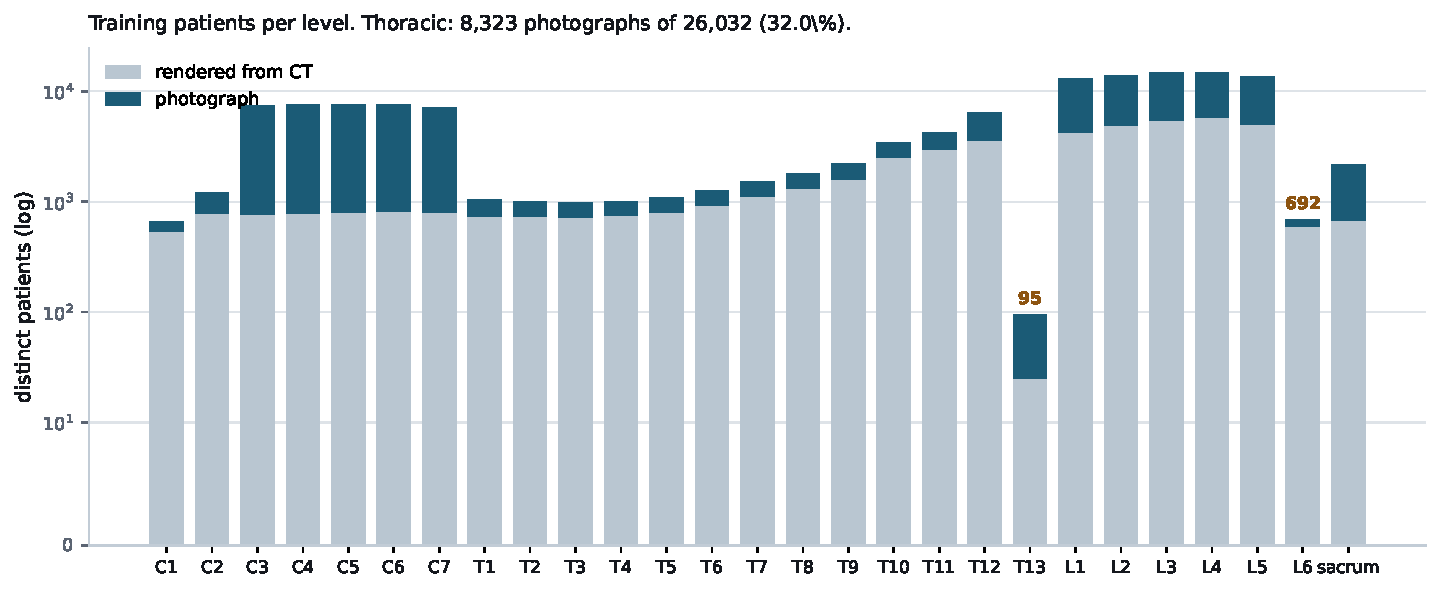
\includegraphics[width=\textwidth]{fig_dataset_levels.pdf}
\caption{Training patients at each level, split by whether the image is a photograph or a rendering of a CT.
The vertical scale is logarithmic. The shape of this figure, not the size of the corpus, is what every
limitation in this paper is downstream of.}
\label{fig:dataset}
\end{figure}

\begin{table}[htbp]\centering
\caption{One limited field, named twice: on the frame's own posterior, and with the chain's ordering
constraint applied. The pixels are identical in both columns of each pair; only the constraint differs.
$n$ is held-out spines. Generated by \texttt{tools/make\_results\_table.py}; nothing in it is typed.}
\label{tab:sweep}
\resizebox{\textwidth}{!}{% GENERATED by tools/make_results_table.py -- do not edit; re-run instead.
\begin{tabular}{llrrrrrrr}
\toprule
& & & \multicolumn{2}{c}{2 vertebrae} & \multicolumn{2}{c}{3 vertebrae} & \multicolumn{2}{c}{4 vertebrae} \\
\cmidrule(lr){4-5}\cmidrule(lr){6-7}\cmidrule(lr){8-9}
Arm & Spine & $n$ & alone & chain & alone & chain & alone & chain \\
\midrule
CT renders, 9-inch field & all & 120 & 72.1 & \textbf{95.2} & 86.8 & \textbf{94.7} & 90.2 & \textbf{94.8} \\
CT renders, 9-inch field & ordinary & 75 & 69.9 & \textbf{94.4} & 85.5 & \textbf{92.8} & 89.2 & \textbf{94.5} \\
CT renders, 9-inch field & lumbosacral & 6 & 76.9 & \textbf{100.0} & 72.7 & \textbf{100.0} & 90.9 & \textbf{100.0} \\
CT renders, 9-inch field & both & 1 & 100.0 & \textbf{100.0} & 100.0 & \textbf{100.0} & 100.0 & \textbf{100.0} \\
CT renders, 9-inch field & unknown & 37 & 74.3 & \textbf{95.9} & 90.8 & \textbf{97.4} & 91.4 & \textbf{94.3} \\
TotalSegmentator renders & all & 522 & 53.3 & \textbf{91.7} & 71.4 & \textbf{91.5} & 82.8 & \textbf{92.5} \\
TotalSegmentator renders & unknown & 522 & 53.3 & \textbf{91.7} & 71.4 & \textbf{91.5} & 82.8 & \textbf{92.5} \\
real radiographs & all & 25 & 78.7 & \textbf{93.6} & 85.7 & \textbf{93.9} & 91.9 & \textbf{100.0} \\
real radiographs & unknown & 25 & 78.7 & \textbf{93.6} & 85.7 & \textbf{93.9} & 91.9 & \textbf{100.0} \\
whole spine, swept from C2 & all & 12 & 9.5 & \textbf{100.0} & 25.0 & \textbf{100.0} & 30.4 & \textbf{100.0} \\
whole spine, swept from C2 & ordinary & 3 & 25.0 & \textbf{100.0} & 33.3 & \textbf{100.0} & 40.0 & \textbf{100.0} \\
whole spine, swept from C2 & unknown & 8 & 6.2 & \textbf{100.0} & 25.0 & \textbf{100.0} & 25.0 & \textbf{100.0} \\
TotalSegmentator, swept from C2 & all & 203 & 18.9 & \textbf{94.0} & 39.5 & \textbf{96.4} & 58.8 & \textbf{97.8} \\
TotalSegmentator, swept from C2 & unknown & 203 & 18.9 & \textbf{94.0} & 39.5 & \textbf{96.4} & 58.8 & \textbf{97.8} \\
\bottomrule
\end{tabular}
}
\end{table}

\begin{table}[htbp]\centering
\caption{Fourteen encoder arms on one common held-out set: the 2,927 patients in the validation split of
every bank and the training split of none, so the banks are comparable. Exact and macro accuracy over 27
classes, with the four levels that separate the arms. Generated; nothing is typed.}
\label{tab:encoders}
\resizebox{\textwidth}{!}{% GENERATED by tools/make_results_table.py -- do not edit; re-run instead.
\begin{tabular}{lrrrrrr}
\toprule
Arm & exact & macro & T12 & L5 & L6 & T13 \\
\midrule
r18\_la\_v2 & 81.1 & 71.3 & 75.1 & 83.4 & 53.0 & 0.0 \\
r18\_la\_v6 & 81.0 & 70.8 & 75.0 & 84.2 & 62.9 & 0.0 \\
r18\_la\_v7 & 80.8 & 71.0 & 73.9 & 79.6 & 72.0 & 0.0 \\
r18\_ce\_v4 & 79.9 & 70.7 & 75.8 & 83.1 & 55.3 & 0.0 \\
r18\_ce\_v3 & 79.7 & 71.0 & 75.7 & 82.2 & 59.1 & 7.1 \\
r18\_ce\_v5c & 79.1 & 70.2 & 74.9 & 80.2 & 55.3 & 0.0 \\
r18\_ce\_v6 & 79.0 & 70.8 & 76.8 & 80.6 & 67.4 & 0.0 \\
r18\_corn\_v6 & 78.9 & 70.5 & 75.8 & 80.4 & 62.1 & 0.0 \\
r18\_ce\_v5 & 78.8 & 70.7 & 76.1 & 76.3 & 62.9 & 0.0 \\
r18\_ce & 78.8 & 70.4 & 71.2 & 78.9 & 64.4 & 0.0 \\
r18\_corn\_v5 & 78.7 & 70.6 & 75.4 & 76.8 & 62.1 & 0.0 \\
r18\_corn\_v5c & 78.7 & 69.9 & 74.7 & 77.8 & 57.6 & 0.0 \\
r18\_corn & 78.4 & 70.0 & 76.9 & 79.9 & 60.6 & 0.0 \\
r18\_ce\_v7 & 77.1 & 69.7 & 71.1 & 74.2 & 73.5 & 0.0 \\
\bottomrule
\end{tabular}
% 2927 patients, 16392 crops, in the val split of every bank and the train split of none
}
\end{table}

\begin{table}[htbp]\centering
\caption{Published figures beside a statement of what each one measures. This is deliberately not a ranking:
registration convergence, label placement conditioned on a correct CT, a questionnaire, a detection score
and a naming accuracy are different quantities, and the third column is the point of the table.}
\label{tab:published}
\resizebox{\textwidth}{!}{% GENERATED by tools/make_results_table.py -- do not edit; re-run instead.
\begin{tabular}{p{4.3cm}p{3.6cm}p{4.4cm}rrl}
\toprule
Method & Setting & What was measured & Value & $n$ & 95\% CI \\
\midrule
\multicolumn{6}{l}{\textbf{Naming one limited field, with and without the chain}\quad\footnotesize The same pixels, named twice: on the frame's own posterior, then with the chain's ordering constraint applied. This is the paper's central comparison.} \\
\midrule
this work, CT renders & 2 vertebrae, all & exact name, frame alone & 72.1 & 484 &  \\
this work, CT renders & 2 vertebrae, all & exact name, on the chain & 95.2 & 484 & [91.6, 98.4] \\
this work, CT renders & 3 vertebrae, all & exact name, frame alone & 86.8 & 720 &  \\
this work, CT renders & 3 vertebrae, all & exact name, on the chain & 94.7 & 720 & [90.8, 98.2] \\
this work, CT renders & 4 vertebrae, all & exact name, frame alone & 90.2 & 904 &  \\
this work, CT renders & 4 vertebrae, all & exact name, on the chain & 94.8 & 904 & [90.8, 98.2] \\
this work, CT renders & the whole chain, all & exact name & 96.7 & 120 & [93.8, 99.1] \\
this work, CT renders & 2 vertebrae, ordinary & exact name, frame alone & 69.9 & 302 &  \\
this work, CT renders & 2 vertebrae, ordinary & exact name, on the chain & 94.4 & 302 & [89.0, 98.4] \\
this work, CT renders & 3 vertebrae, ordinary & exact name, frame alone & 85.5 & 447 &  \\
this work, CT renders & 3 vertebrae, ordinary & exact name, on the chain & 92.8 & 447 & [86.9, 97.4] \\
this work, CT renders & 4 vertebrae, ordinary & exact name, frame alone & 89.2 & 564 &  \\
this work, CT renders & 4 vertebrae, ordinary & exact name, on the chain & 94.5 & 564 & [88.9, 98.6] \\
this work, CT renders & the whole chain, ordinary & exact name & 95.9 & 75 & [91.9, 99.0] \\
this work, CT renders & 2 vertebrae, lumbosacral & exact name, frame alone & 76.9 & 26 &  \\
this work, CT renders & 2 vertebrae, lumbosacral & exact name, on the chain & 100.0 & 26 & [100.0, 100.0] \\
this work, CT renders & 3 vertebrae, lumbosacral & exact name, frame alone & 72.7 & 33 &  \\
this work, CT renders & 3 vertebrae, lumbosacral & exact name, on the chain & 100.0 & 33 & [100.0, 100.0] \\
this work, CT renders & 4 vertebrae, lumbosacral & exact name, frame alone & 90.9 & 44 &  \\
this work, CT renders & 4 vertebrae, lumbosacral & exact name, on the chain & 100.0 & 44 & [100.0, 100.0] \\
this work, CT renders & the whole chain, lumbosacral & exact name & 100.0 & 6 & [100.0, 100.0] \\
this work, CT renders & 2 vertebrae, thoracolumbar & exact name, frame alone & 100.0 & 4 &  \\
this work, CT renders & 2 vertebrae, thoracolumbar & exact name, on the chain & 100.0 & 4 & [100.0, 100.0] \\
this work, CT renders & 3 vertebrae, thoracolumbar & exact name, frame alone & 100.0 & 6 &  \\
this work, CT renders & 3 vertebrae, thoracolumbar & exact name, on the chain & 100.0 & 6 & [100.0, 100.0] \\
this work, CT renders & 4 vertebrae, thoracolumbar & exact name, frame alone & 100.0 & 8 &  \\
this work, CT renders & 4 vertebrae, thoracolumbar & exact name, on the chain & 100.0 & 8 & [100.0, 100.0] \\
this work, CT renders & the whole chain, thoracolumbar & exact name & 100.0 & 1 & [100.0, 100.0] \\
this work, CT renders & 2 vertebrae, both & exact name, frame alone & 100.0 & 4 &  \\
this work, CT renders & 2 vertebrae, both & exact name, on the chain & 100.0 & 4 & [100.0, 100.0] \\
this work, CT renders & 3 vertebrae, both & exact name, frame alone & 100.0 & 6 &  \\
this work, CT renders & 3 vertebrae, both & exact name, on the chain & 100.0 & 6 & [100.0, 100.0] \\
this work, CT renders & 4 vertebrae, both & exact name, frame alone & 100.0 & 8 &  \\
this work, CT renders & 4 vertebrae, both & exact name, on the chain & 100.0 & 8 & [100.0, 100.0] \\
this work, CT renders & the whole chain, both & exact name & 100.0 & 1 & [100.0, 100.0] \\
this work, CT renders, 1-body overlap & 2 vertebrae, all & exact name, frame alone & 72.7 & 476 &  \\
this work, CT renders, 1-body overlap & 2 vertebrae, all & exact name, on the chain & 95.2 & 476 & [91.6, 98.1] \\
this work, CT renders, 1-body overlap & 3 vertebrae, all & exact name, frame alone & 84.7 & 720 &  \\
this work, CT renders, 1-body overlap & 3 vertebrae, all & exact name, on the chain & 93.6 & 720 & [89.3, 97.5] \\
this work, CT renders, 1-body overlap & 4 vertebrae, all & exact name, frame alone & 90.1 & 912 &  \\
this work, CT renders, 1-body overlap & 4 vertebrae, all & exact name, on the chain & 95.7 & 912 & [92.1, 98.7] \\
this work, CT renders, 1-body overlap & the whole chain, all & exact name & 96.7 & 120 & [94.0, 99.0] \\
this work, CT renders, 1-body overlap & 2 vertebrae, ordinary & exact name, frame alone & 72.1 & 294 &  \\
this work, CT renders, 1-body overlap & 2 vertebrae, ordinary & exact name, on the chain & 94.2 & 294 & [89.0, 98.0] \\
this work, CT renders, 1-body overlap & 3 vertebrae, ordinary & exact name, frame alone & 85.2 & 459 &  \\
this work, CT renders, 1-body overlap & 3 vertebrae, ordinary & exact name, on the chain & 92.6 & 459 & [86.4, 97.6] \\
this work, CT renders, 1-body overlap & 4 vertebrae, ordinary & exact name, frame alone & 89.6 & 556 &  \\
this work, CT renders, 1-body overlap & 4 vertebrae, ordinary & exact name, on the chain & 96.0 & 556 & [91.7, 99.3] \\
this work, CT renders, 1-body overlap & the whole chain, ordinary & exact name & 96.0 & 75 & [92.3, 98.9] \\
this work, CT renders, 1-body overlap & 2 vertebrae, lumbosacral & exact name, frame alone & 58.3 & 24 &  \\
this work, CT renders, 1-body overlap & 2 vertebrae, lumbosacral & exact name, on the chain & 91.7 & 24 & [75.0, 100.0] \\
this work, CT renders, 1-body overlap & 3 vertebrae, lumbosacral & exact name, frame alone & 75.0 & 36 &  \\
this work, CT renders, 1-body overlap & 3 vertebrae, lumbosacral & exact name, on the chain & 100.0 & 36 & [100.0, 100.0] \\
this work, CT renders, 1-body overlap & 4 vertebrae, lumbosacral & exact name, frame alone & 75.0 & 48 &  \\
this work, CT renders, 1-body overlap & 4 vertebrae, lumbosacral & exact name, on the chain & 97.9 & 48 & [93.8, 100.0] \\
this work, CT renders, 1-body overlap & the whole chain, lumbosacral & exact name & 96.0 & 6 & [87.0, 100.0] \\
this work, CT renders, 1-body overlap & 2 vertebrae, thoracolumbar & exact name, frame alone & 100.0 & 4 &  \\
this work, CT renders, 1-body overlap & 2 vertebrae, thoracolumbar & exact name, on the chain & 100.0 & 4 & [100.0, 100.0] \\
this work, CT renders, 1-body overlap & 3 vertebrae, thoracolumbar & exact name, frame alone & 100.0 & 6 &  \\
this work, CT renders, 1-body overlap & 3 vertebrae, thoracolumbar & exact name, on the chain & 100.0 & 6 & [100.0, 100.0] \\
this work, CT renders, 1-body overlap & 4 vertebrae, thoracolumbar & exact name, frame alone & 100.0 & 8 &  \\
this work, CT renders, 1-body overlap & 4 vertebrae, thoracolumbar & exact name, on the chain & 100.0 & 8 & [100.0, 100.0] \\
this work, CT renders, 1-body overlap & the whole chain, thoracolumbar & exact name & 100.0 & 1 & [100.0, 100.0] \\
this work, CT renders, 1-body overlap & 2 vertebrae, both & exact name, frame alone & 50.0 & 4 &  \\
this work, CT renders, 1-body overlap & 2 vertebrae, both & exact name, on the chain & 100.0 & 4 & [100.0, 100.0] \\
this work, CT renders, 1-body overlap & 3 vertebrae, both & exact name, frame alone & 100.0 & 6 &  \\
this work, CT renders, 1-body overlap & 3 vertebrae, both & exact name, on the chain & 100.0 & 6 & [100.0, 100.0] \\
this work, CT renders, 1-body overlap & 4 vertebrae, both & exact name, frame alone & 100.0 & 8 &  \\
this work, CT renders, 1-body overlap & 4 vertebrae, both & exact name, on the chain & 100.0 & 8 & [100.0, 100.0] \\
this work, CT renders, 1-body overlap & the whole chain, both & exact name & 100.0 & 1 & [100.0, 100.0] \\
this work, real radiographs & 2 vertebrae, all & exact name, frame alone & 78.7 & 94 &  \\
this work, real radiographs & 2 vertebrae, all & exact name, on the chain & 93.6 & 94 & [85.4, 100.0] \\
this work, real radiographs & 3 vertebrae, all & exact name, frame alone & 85.7 & 147 &  \\
this work, real radiographs & 3 vertebrae, all & exact name, on the chain & 93.9 & 147 & [87.5, 100.0] \\
this work, real radiographs & 4 vertebrae, all & exact name, frame alone & 91.9 & 148 &  \\
this work, real radiographs & 4 vertebrae, all & exact name, on the chain & 100.0 & 148 & [100.0, 100.0] \\
this work, real radiographs & the whole chain, all & exact name & 100.0 & 25 & [100.0, 100.0] \\
this work, whole-spine, swept from C2 & 2 vertebrae, all & exact name, frame alone & 9.5 & 42 &  \\
this work, whole-spine, swept from C2 & 2 vertebrae, all & exact name, on the chain & 100.0 & 42 & [100.0, 100.0] \\
this work, whole-spine, swept from C2 & 3 vertebrae, all & exact name, frame alone & 25.0 & 72 &  \\
this work, whole-spine, swept from C2 & 3 vertebrae, all & exact name, on the chain & 100.0 & 72 & [100.0, 100.0] \\
this work, whole-spine, swept from C2 & 4 vertebrae, all & exact name, frame alone & 30.4 & 92 &  \\
this work, whole-spine, swept from C2 & 4 vertebrae, all & exact name, on the chain & 100.0 & 92 & [100.0, 100.0] \\
this work, whole-spine, swept from C2 & the whole chain, all & exact name & 100.0 & 12 & [100.0, 100.0] \\
this work, whole-spine, swept from C2 & 2 vertebrae, ordinary & exact name, frame alone & 25.0 & 8 &  \\
this work, whole-spine, swept from C2 & 2 vertebrae, ordinary & exact name, on the chain & 100.0 & 8 & [100.0, 100.0] \\
this work, whole-spine, swept from C2 & 3 vertebrae, ordinary & exact name, frame alone & 33.3 & 18 &  \\
this work, whole-spine, swept from C2 & 3 vertebrae, ordinary & exact name, on the chain & 100.0 & 18 & [100.0, 100.0] \\
this work, whole-spine, swept from C2 & 4 vertebrae, ordinary & exact name, frame alone & 40.0 & 20 &  \\
this work, whole-spine, swept from C2 & 4 vertebrae, ordinary & exact name, on the chain & 100.0 & 20 & [100.0, 100.0] \\
this work, whole-spine, swept from C2 & the whole chain, ordinary & exact name & 100.0 & 3 & [100.0, 100.0] \\
this work, whole-spine, swept from C2 & 2 vertebrae, thoracolumbar & exact name, frame alone & 0.0 & 2 &  \\
this work, whole-spine, swept from C2 & 2 vertebrae, thoracolumbar & exact name, on the chain & 100.0 & 2 & [100.0, 100.0] \\
this work, whole-spine, swept from C2 & 3 vertebrae, thoracolumbar & exact name, frame alone & 0.0 & 6 &  \\
this work, whole-spine, swept from C2 & 3 vertebrae, thoracolumbar & exact name, on the chain & 100.0 & 6 & [100.0, 100.0] \\
this work, whole-spine, swept from C2 & 4 vertebrae, thoracolumbar & exact name, frame alone & 50.0 & 8 &  \\
this work, whole-spine, swept from C2 & 4 vertebrae, thoracolumbar & exact name, on the chain & 100.0 & 8 & [100.0, 100.0] \\
this work, whole-spine, swept from C2 & the whole chain, thoracolumbar & exact name & 100.0 & 1 & [100.0, 100.0] \\
this work, TotalSegmentator renders (1170 CTs, none in any bank) & 2 vertebrae, all & exact name, frame alone & 53.3 & 2038 &  \\
this work, TotalSegmentator renders (1170 CTs, none in any bank) & 2 vertebrae, all & exact name, on the chain & 91.7 & 2038 & [89.4, 93.8] \\
this work, TotalSegmentator renders (1170 CTs, none in any bank) & 3 vertebrae, all & exact name, frame alone & 71.4 & 3039 &  \\
this work, TotalSegmentator renders (1170 CTs, none in any bank) & 3 vertebrae, all & exact name, on the chain & 91.5 & 3039 & [89.3, 93.6] \\
this work, TotalSegmentator renders (1170 CTs, none in any bank) & 4 vertebrae, all & exact name, frame alone & 82.8 & 3208 &  \\
this work, TotalSegmentator renders (1170 CTs, none in any bank) & 4 vertebrae, all & exact name, on the chain & 92.5 & 3208 & [90.2, 94.6] \\
this work, TotalSegmentator renders (1170 CTs, none in any bank) & the whole chain, all & exact name & 91.9 & 522 & [89.7, 93.8] \\
this work, TotalSegmentator whole-spine, swept from C2 & 2 vertebrae, all & exact name, frame alone & 18.9 & 814 &  \\
this work, TotalSegmentator whole-spine, swept from C2 & 2 vertebrae, all & exact name, on the chain & 94.0 & 814 & [91.5, 96.4] \\
this work, TotalSegmentator whole-spine, swept from C2 & 3 vertebrae, all & exact name, frame alone & 39.5 & 1206 &  \\
this work, TotalSegmentator whole-spine, swept from C2 & 3 vertebrae, all & exact name, on the chain & 96.4 & 1206 & [94.2, 98.3] \\
this work, TotalSegmentator whole-spine, swept from C2 & 4 vertebrae, all & exact name, frame alone & 58.8 & 1404 &  \\
this work, TotalSegmentator whole-spine, swept from C2 & 4 vertebrae, all & exact name, on the chain & 97.8 & 1404 & [96.0, 99.3] \\
this work, TotalSegmentator whole-spine, swept from C2 & the whole chain, all & exact name & 93.8 & 203 & [91.4, 96.1] \\
this work, CT renders, protocol as written (fixed 2-body step) & 2 vertebrae, all & exact name, frame alone & 69.9 & 482 &  \\
this work, CT renders, protocol as written (fixed 2-body step) & 2 vertebrae, all & exact name, on the chain & 93.6 & 482 & [89.5, 97.3] \\
this work, CT renders, protocol as written (fixed 2-body step) & 3 vertebrae, all & exact name, frame alone & 87.5 & 720 &  \\
this work, CT renders, protocol as written (fixed 2-body step) & 3 vertebrae, all & exact name, on the chain & 94.7 & 720 & [90.6, 98.0] \\
this work, CT renders, protocol as written (fixed 2-body step) & 4 vertebrae, all & exact name, frame alone & 88.2 & 908 &  \\
this work, CT renders, protocol as written (fixed 2-body step) & 4 vertebrae, all & exact name, on the chain & 93.9 & 908 & [90.0, 97.5] \\
this work, CT renders, protocol as written (fixed 2-body step) & the whole chain, all & exact name & 95.5 & 120 & [91.7, 98.7] \\
this work, CT renders, protocol as written (fixed 2-body step) & 2 vertebrae, ordinary & exact name, frame alone & 68.5 & 302 &  \\
this work, CT renders, protocol as written (fixed 2-body step) & 2 vertebrae, ordinary & exact name, on the chain & 92.4 & 302 & [86.6, 97.2] \\
this work, CT renders, protocol as written (fixed 2-body step) & 3 vertebrae, ordinary & exact name, frame alone & 86.5 & 444 &  \\
this work, CT renders, protocol as written (fixed 2-body step) & 3 vertebrae, ordinary & exact name, on the chain & 94.1 & 444 & [89.0, 98.3] \\
this work, CT renders, protocol as written (fixed 2-body step) & 4 vertebrae, ordinary & exact name, frame alone & 86.8 & 568 &  \\
this work, CT renders, protocol as written (fixed 2-body step) & 4 vertebrae, ordinary & exact name, on the chain & 92.4 & 568 & [86.7, 97.2] \\
this work, CT renders, protocol as written (fixed 2-body step) & the whole chain, ordinary & exact name & 94.5 & 75 & [88.8, 98.9] \\
this work, CT renders, protocol as written (fixed 2-body step) & 2 vertebrae, lumbosacral & exact name, frame alone & 76.9 & 26 &  \\
this work, CT renders, protocol as written (fixed 2-body step) & 2 vertebrae, lumbosacral & exact name, on the chain & 100.0 & 26 & [100.0, 100.0] \\
this work, CT renders, protocol as written (fixed 2-body step) & 3 vertebrae, lumbosacral & exact name, frame alone & 83.3 & 36 &  \\
this work, CT renders, protocol as written (fixed 2-body step) & 3 vertebrae, lumbosacral & exact name, on the chain & 100.0 & 36 & [100.0, 100.0] \\
this work, CT renders, protocol as written (fixed 2-body step) & 4 vertebrae, lumbosacral & exact name, frame alone & 90.9 & 44 &  \\
this work, CT renders, protocol as written (fixed 2-body step) & 4 vertebrae, lumbosacral & exact name, on the chain & 100.0 & 44 & [100.0, 100.0] \\
this work, CT renders, protocol as written (fixed 2-body step) & the whole chain, lumbosacral & exact name & 100.0 & 6 & [100.0, 100.0] \\
this work, CT renders, protocol as written (fixed 2-body step) & 2 vertebrae, thoracolumbar & exact name, frame alone & 50.0 & 4 &  \\
this work, CT renders, protocol as written (fixed 2-body step) & 2 vertebrae, thoracolumbar & exact name, on the chain & 100.0 & 4 & [100.0, 100.0] \\
this work, CT renders, protocol as written (fixed 2-body step) & 3 vertebrae, thoracolumbar & exact name, frame alone & 100.0 & 6 &  \\
this work, CT renders, protocol as written (fixed 2-body step) & 3 vertebrae, thoracolumbar & exact name, on the chain & 100.0 & 6 & [100.0, 100.0] \\
this work, CT renders, protocol as written (fixed 2-body step) & 4 vertebrae, thoracolumbar & exact name, frame alone & 100.0 & 8 &  \\
this work, CT renders, protocol as written (fixed 2-body step) & 4 vertebrae, thoracolumbar & exact name, on the chain & 100.0 & 8 & [100.0, 100.0] \\
this work, CT renders, protocol as written (fixed 2-body step) & the whole chain, thoracolumbar & exact name & 100.0 & 1 & [100.0, 100.0] \\
this work, CT renders, protocol as written (fixed 2-body step) & 2 vertebrae, both & exact name, frame alone & 100.0 & 4 &  \\
this work, CT renders, protocol as written (fixed 2-body step) & 2 vertebrae, both & exact name, on the chain & 100.0 & 4 & [100.0, 100.0] \\
this work, CT renders, protocol as written (fixed 2-body step) & 3 vertebrae, both & exact name, frame alone & 100.0 & 6 &  \\
this work, CT renders, protocol as written (fixed 2-body step) & 3 vertebrae, both & exact name, on the chain & 100.0 & 6 & [100.0, 100.0] \\
this work, CT renders, protocol as written (fixed 2-body step) & 4 vertebrae, both & exact name, frame alone & 100.0 & 8 &  \\
this work, CT renders, protocol as written (fixed 2-body step) & 4 vertebrae, both & exact name, on the chain & 100.0 & 8 & [100.0, 100.0] \\
this work, CT renders, protocol as written (fixed 2-body step) & the whole chain, both & exact name & 100.0 & 1 & [100.0, 100.0] \\
\midrule
\multicolumn{6}{l}{\textbf{Encoder arms on one common held-out set}\quad\footnotesize Every arm scored on the cases in the validation split of EVERY bank and the training split of none, so the banks are comparable.} \\
\midrule
r18\_ce & 2927 patients, one common set & exact name, single crop & 78.8 & 16392 &  \\
r18\_ce & class L6 & exact name, single crop & 64.4 & 105 & [55.9, 72.0] \\
r18\_ce & class T13 & exact name, single crop & 0.0 & 12 & [0.0, 21.5] \\
r18\_ce & class T12 & exact name, single crop & 71.2 & 691 & [67.8, 74.4] \\
r18\_ce & class L5 & exact name, single crop & 78.9 & 1492 & [76.8, 80.9] \\
r18\_corn & 2927 patients, one common set & exact name, single crop & 78.4 & 16392 &  \\
r18\_corn & class L6 & exact name, single crop & 60.6 & 105 & [52.1, 68.5] \\
r18\_corn & class T13 & exact name, single crop & 0.0 & 12 & [0.0, 21.5] \\
r18\_corn & class T12 & exact name, single crop & 76.9 & 691 & [73.7, 79.9] \\
r18\_corn & class L5 & exact name, single crop & 79.9 & 1492 & [77.8, 81.8] \\
r18\_la\_v2 & 2927 patients, one common set & exact name, single crop & 81.1 & 16392 &  \\
r18\_la\_v2 & class L6 & exact name, single crop & 53.0 & 105 & [44.5, 61.3] \\
r18\_la\_v2 & class T13 & exact name, single crop & 0.0 & 12 & [0.0, 21.5] \\
r18\_la\_v2 & class T12 & exact name, single crop & 75.1 & 691 & [71.9, 78.2] \\
r18\_la\_v2 & class L5 & exact name, single crop & 83.4 & 1492 & [81.5, 85.2] \\
r18\_ce\_v3 & 2927 patients, one common set & exact name, single crop & 79.7 & 16392 &  \\
r18\_ce\_v3 & class L6 & exact name, single crop & 59.1 & 105 & [50.6, 67.1] \\
r18\_ce\_v3 & class T13 & exact name, single crop & 7.1 & 12 & [1.3, 31.5] \\
r18\_ce\_v3 & class T12 & exact name, single crop & 75.7 & 691 & [72.4, 78.7] \\
r18\_ce\_v3 & class L5 & exact name, single crop & 82.2 & 1492 & [80.2, 84.0] \\
r18\_ce\_v4 & 2927 patients, one common set & exact name, single crop & 79.9 & 16392 &  \\
r18\_ce\_v4 & class L6 & exact name, single crop & 55.3 & 105 & [46.8, 63.5] \\
r18\_ce\_v4 & class T13 & exact name, single crop & 0.0 & 12 & [0.0, 21.5] \\
r18\_ce\_v4 & class T12 & exact name, single crop & 75.8 & 691 & [72.6, 78.8] \\
r18\_ce\_v4 & class L5 & exact name, single crop & 83.1 & 1492 & [81.2, 84.9] \\
r18\_ce\_v5 & 2927 patients, one common set & exact name, single crop & 78.8 & 16392 &  \\
r18\_ce\_v5 & class L6 & exact name, single crop & 62.9 & 105 & [54.4, 70.7] \\
r18\_ce\_v5 & class T13 & exact name, single crop & 0.0 & 12 & [0.0, 21.5] \\
r18\_ce\_v5 & class T12 & exact name, single crop & 76.1 & 691 & [72.9, 79.1] \\
r18\_ce\_v5 & class L5 & exact name, single crop & 76.3 & 1492 & [74.1, 78.3] \\
r18\_corn\_v5 & 2927 patients, one common set & exact name, single crop & 78.7 & 16392 &  \\
r18\_corn\_v5 & class L6 & exact name, single crop & 62.1 & 105 & [53.6, 69.9] \\
r18\_corn\_v5 & class T13 & exact name, single crop & 0.0 & 12 & [0.0, 21.5] \\
r18\_corn\_v5 & class T12 & exact name, single crop & 75.4 & 691 & [72.1, 78.4] \\
r18\_corn\_v5 & class L5 & exact name, single crop & 76.8 & 1492 & [74.6, 78.8] \\
r18\_ce\_v5c & 2927 patients, one common set & exact name, single crop & 79.1 & 16392 &  \\
r18\_ce\_v5c & class L6 & exact name, single crop & 55.3 & 105 & [46.8, 63.5] \\
r18\_ce\_v5c & class T13 & exact name, single crop & 0.0 & 12 & [0.0, 21.5] \\
r18\_ce\_v5c & class T12 & exact name, single crop & 74.9 & 691 & [71.6, 77.9] \\
r18\_ce\_v5c & class L5 & exact name, single crop & 80.2 & 1492 & [78.2, 82.2] \\
r18\_corn\_v5c & 2927 patients, one common set & exact name, single crop & 78.7 & 16392 &  \\
r18\_corn\_v5c & class L6 & exact name, single crop & 57.6 & 105 & [49.0, 65.7] \\
r18\_corn\_v5c & class T13 & exact name, single crop & 0.0 & 12 & [0.0, 21.5] \\
r18\_corn\_v5c & class T12 & exact name, single crop & 74.7 & 691 & [71.4, 77.8] \\
r18\_corn\_v5c & class L5 & exact name, single crop & 77.8 & 1492 & [75.7, 79.8] \\
r18\_ce\_v6 & 2927 patients, one common set & exact name, single crop & 79.0 & 16392 &  \\
r18\_ce\_v6 & class L6 & exact name, single crop & 67.4 & 105 & [59.0, 74.8] \\
r18\_ce\_v6 & class T13 & exact name, single crop & 0.0 & 12 & [0.0, 21.5] \\
r18\_ce\_v6 & class T12 & exact name, single crop & 76.8 & 691 & [73.6, 79.7] \\
r18\_ce\_v6 & class L5 & exact name, single crop & 80.6 & 1492 & [78.6, 82.5] \\
r18\_la\_v6 & 2927 patients, one common set & exact name, single crop & 81.0 & 16392 &  \\
r18\_la\_v6 & class L6 & exact name, single crop & 62.9 & 105 & [54.4, 70.7] \\
r18\_la\_v6 & class T13 & exact name, single crop & 0.0 & 12 & [0.0, 21.5] \\
r18\_la\_v6 & class T12 & exact name, single crop & 75.0 & 691 & [71.7, 78.0] \\
r18\_la\_v6 & class L5 & exact name, single crop & 84.2 & 1492 & [82.3, 86.0] \\
r18\_corn\_v6 & 2927 patients, one common set & exact name, single crop & 78.9 & 16392 &  \\
r18\_corn\_v6 & class L6 & exact name, single crop & 62.1 & 105 & [53.6, 69.9] \\
r18\_corn\_v6 & class T13 & exact name, single crop & 0.0 & 12 & [0.0, 21.5] \\
r18\_corn\_v6 & class T12 & exact name, single crop & 75.8 & 691 & [72.6, 78.8] \\
r18\_corn\_v6 & class L5 & exact name, single crop & 80.4 & 1492 & [78.4, 82.3] \\
r18\_ce\_v7 & 2927 patients, one common set & exact name, single crop & 77.1 & 16392 &  \\
r18\_ce\_v7 & class L6 & exact name, single crop & 73.5 & 105 & [65.4, 80.3] \\
r18\_ce\_v7 & class T13 & exact name, single crop & 0.0 & 12 & [0.0, 21.5] \\
r18\_ce\_v7 & class T12 & exact name, single crop & 71.1 & 691 & [67.7, 74.3] \\
r18\_ce\_v7 & class L5 & exact name, single crop & 74.2 & 1492 & [72.0, 76.4] \\
r18\_la\_v7 & 2927 patients, one common set & exact name, single crop & 80.8 & 16392 &  \\
r18\_la\_v7 & class L6 & exact name, single crop & 72.0 & 105 & [63.8, 78.9] \\
r18\_la\_v7 & class T13 & exact name, single crop & 0.0 & 12 & [0.0, 21.5] \\
r18\_la\_v7 & class T12 & exact name, single crop & 73.9 & 691 & [70.6, 77.0] \\
r18\_la\_v7 & class L5 & exact name, single crop & 79.6 & 1492 & [77.5, 81.5] \\
\midrule
\multicolumn{6}{l}{\textbf{Published methods, rebuilt and trained on these data}\quad\footnotesize Rebuilt from stated architectures because none releases code or weights.} \\
\midrule
cina & no map, mean & exact name, held-out half & 41.1 & 20865 &  \\
cina & with the map, mean & exact name, held-out half & 43.2 & 20865 &  \\
kim & no map, mean & exact name, held-out half & 15.7 & 20865 &  \\
kim & with the map, mean & exact name, held-out half & 16.4 & 20865 &  \\
ours & no map, mean & exact name, held-out half & 75.7 & 20865 &  \\
ours & with the map, mean & exact name, held-out half & 79.6 & 20865 &  \\
vertx & no map, mean & exact name, held-out half & 0.3 & 20865 &  \\
vertx & with the map, mean & exact name, held-out half & 2.0 & 20865 &  \\
cina+kim & with the map, mean & exact name, held-out half & 42.1 & 20865 &  \\
cina+kim & with the map, vote & exact name, held-out half & 39.6 & 20865 &  \\
cina+ours & with the map, mean & exact name, held-out half & 64.9 & 20865 &  \\
cina+ours & with the map, vote & exact name, held-out half & 72.9 & 20865 &  \\
cina+vertx & with the map, mean & exact name, held-out half & 43.2 & 20865 &  \\
cina+vertx & with the map, vote & exact name, held-out half & 41.4 & 20865 &  \\
kim+ours & with the map, mean & exact name, held-out half & 77.0 & 20865 &  \\
kim+ours & with the map, vote & exact name, held-out half & 75.8 & 20865 &  \\
kim+vertx & with the map, mean & exact name, held-out half & 17.3 & 20865 &  \\
kim+vertx & with the map, vote & exact name, held-out half & 16.4 & 20865 &  \\
ours+vertx & with the map, mean & exact name, held-out half & 77.8 & 20865 &  \\
ours+vertx & with the map, vote & exact name, held-out half & 77.4 & 20865 &  \\
cina+kim+ours & with the map, mean & exact name, held-out half & 63.7 & 20865 &  \\
cina+kim+ours & with the map, vote & exact name, held-out half & 71.9 & 20865 &  \\
cina+kim+vertx & with the map, mean & exact name, held-out half & 42.1 & 20865 &  \\
cina+kim+vertx & with the map, vote & exact name, held-out half & 17.9 & 20865 &  \\
cina+ours+vertx & with the map, mean & exact name, held-out half & 65.5 & 20865 &  \\
cina+ours+vertx & with the map, vote & exact name, held-out half & 72.6 & 20865 &  \\
kim+ours+vertx & with the map, mean & exact name, held-out half & 76.1 & 20865 &  \\
kim+ours+vertx & with the map, vote & exact name, held-out half & 20.9 & 20865 &  \\
cina+kim+ours+vertx & with the map, mean & exact name, held-out half & 64.2 & 20865 &  \\
cina+kim+ours+vertx & with the map, vote & exact name, held-out half & 44.7 & 20865 &  \\
BUU five-slot detector (rebuilt) & whole lumbar film & per-level assignment & -- & -- &  \\
\midrule
\multicolumn{6}{l}{\textbf{Published figures, as each paper reports them}\quad\footnotesize NOT a ranking. Each cell is that study's own metric on its own cohort at its own field of view; the measure column is the point of this block.} \\
\midrule
LevelCheck (Otake 2012) & fluoroscopy, 50,000 simulated trials & registration converged, mean projection distance < 5 mm & 99.998 & -- &  \\
LevelCheck (De Silva 2016) & 398 intraoperative radiographs & label inside the correct body, GIVEN a correctly labelled CT & 100 & 398 &  \\
LevelCheck (De Silva 2016) & 398 cases, 3 surgeons rating independently & questionnaire: 'helpful' & 42.2 & 398 &  \\
Surgeons + LevelCheck (Manbachi 2018) & 62 deliberately difficult C-arm films, 5 surgeons & correct level named, human plus machine & 97.6 & 62 &  \\
Surgeons unaided (Manbachi 2018) & 62 deliberately difficult C-arm films, 5 surgeons & correct level named & 69.6 & 62 &  \\
MVMS (Huang 2022) & 13 cadavers, long-film, ~64 cm field & vertebra labelling accuracy & 88.3 & 100 &  \\
MVMS (Huang 2022) & same images & detection F1 & >96 & 100 &  \\
Cina 2021 & 195 whole lumbar films, sacrum usually in frame & per-vertebra correct name & 98.4 & 195 &  \\
VertXNet (2024) & whole spine & Panoptic Quality & 0.88 & -- &  \\
VERIDAH (2026) & 3-D CT volumes, ordered chain supplied & subjects perfectly labelled & 99.18 & -- &  \\
\bottomrule
\end{tabular}
}
\end{table}

\begin{table}[htbp]\centering
\caption{The protocol as written and what was tried on it. Every row is the same 120 held-out CT renders
with the same photometric draws; the first row is the jittered-step reference, the second the fixed
sacrum-to-cranial step a radiographer is told to make, and the rest add one panoramic-stitching change at
a time at the stated overlap. Generated; nothing is typed.}
\label{tab:protocol}
\resizebox{\textwidth}{!}{% GENERATED by tools/make_results_table.py -- do not edit; re-run instead.
\begin{tabular}{lrrrrrrr}
\toprule
Arm & overlap & exposures & chain complete & duplicates/spine & 2 vert. & 3 vert. & 4 vert. \\
\midrule
jittered step (reference) & 2 & 3.42 & 97.5 & 0.000 & 95.2 & 94.7 & 94.8 \\
fixed step, as written & 2 & 3.39 & 95.0 & 0.042 & 93.6 & 94.7 & 93.9 \\
fixed step, final move under half a body refused & 2 & 3.32 & 100.0 & 0.000 & 94.7 & 96.3 & 94.2 \\
fixed step, last link searched to zero step & 2 & 3.39 & 100.0 & 0.000 & 94.4 & 95.4 & 94.9 \\
jittered step, last link searched to zero step & 2 & 3.42 & 100.0 & 0.000 & 95.2 & 95.1 & 95.0 \\
+ global link solve & 2 & 3.39 & 92.5 & 0.058 & 92.1 & 92.5 & 92.1 \\
+ phase-correlation seed & 2 & 3.39 & 95.0 & 0.000 & 94.0 & 94.3 & 94.1 \\
+ ECC placement & 2 & 3.39 & 95.0 & 0.042 & 93.6 & 94.7 & 93.9 \\
+ all three & 2 & 3.39 & 92.5 & 0.067 & 91.3 & 91.7 & 91.6 \\
fixed step & 3 & 4.80 & 90.8 & 0.033 & 95.0 & 92.8 & 95.0 \\
+ global link solve & 3 & 4.80 & 91.7 & 0.083 & 93.2 & 91.4 & 92.4 \\
fixed step & 4 & 9.43 & 83.3 & 0.117 & 93.9 & 94.6 & 95.2 \\
+ global link solve & 4 & 9.43 & 90.0 & 0.067 & 94.1 & 94.4 & 94.4 \\
+ all three & 4 & 9.43 & 90.8 & 0.050 & 94.4 & 94.4 & 94.7 \\
\bottomrule
\end{tabular}
% 120 held-out spines in every row; 2/3/4 vert. = exact name on the chain
}
\end{table}

\section*{Figure Legends}
\noindent\textbf{Figure 1.} The report's argument, drawn. The same field of view at the same height above the sacrum holds L4--L2 in an ordinary spine and L5--L3 in a spine with a lumbarised S1; the report concludes that absolute naming is underdetermined. The figure is the claim, not data.

\noindent\textbf{Figure 2.} Exact vertebra naming by the report's field-of-view state, split by real film versus CT render and by anomalous versus ordinary spine, with Wilson 95\% CIs and vertebra counts. Left, bank v2; right, bank v5 (30\% pseudolabelled crops). Dotted line, chance for the scored label distribution.

\noindent\textbf{Figure 3.} Per-level accuracy inside the isolated stack, L1--L6, both banks. Shaded, the levels the report called exchangeable.

\noindent\textbf{Figure 4.} Left, signed ordinal error of every isolated-stack error (v2); $\pm0.5$ is a variant class confused with its neighbour. Right, the shape of error within a window.

\noindent\textbf{Figure 5.} Balanced accuracy of a linear probe for four spine classes against window length, for windows containing neither junction and windows containing one, each with its shuffled-label control. Marker size is proportional to window count.

\noindent\textbf{Figure 6.} Left, AUC of each geometric index on real lateral and anteroposterior films for six-lumbar and four-lumbar spines. Right, the Wigh index of the lowest body on 3,600 lateral films with the report's ``normal L5'' band shaded.

\noindent\textbf{Figure 7.} The serial sweep. Left, exact naming against the number of vertebrae in a limited-field frame, for each spine class: dashed, the frame named on its own pixels; solid, the same frame registered onto the sweep. Right, the same comparison against the physical field of each swept frame, with the share of spines whose chain of vertebrae came out complete printed under each. Drawn by \texttt{tools/make\_sweep\_figure.py} from \texttt{SWEEP\_TABLE.json}.

\medskip


\clearpage
% ------------------------------------------------------------------------------------------------ SUPPLEMENT

\bibliographystyle{unsrtnat}
\bibliography{refs}

\end{document}
